\documentclass[a4paper, 10pt]{article}
\hyphenpenalty=8000
\textwidth=125mm
\textheight=185mm

\usepackage{graphicx} % para insertar imágenes
\usepackage{alltt}    % para describir código y algoritmos
\usepackage{amsmath}  % para expresiones matemáticas
\usepackage[hidelinks, pdftex]{hyperref} % para enlaces
\pagenumbering{arabic}
\setcounter{page}{1}
\renewcommand{\thefootnote}{\fnsymbol{footnote}}
\newcommand{\doi}[1]{\href{https://doi.org/#1}{\texttt{https://doi.org/#1}}}

\begin{document}

\begin{center}

\LARGE
\textbf{Análisis del Conjunto de Datos California Housing}\footnote{Este trabajo forma parte de las actividades del curso de Ingeniería Informática.}\\[6pt]
\small
\textbf{Critian Orozco, Marlon Caviedes, Alan Miranda}\\[6pt]
Infotep\\
\texttt{}\\[6pt]
\end{center}

\begin{abstract}
Este informe expone un estudio exploratorio del conjunto de datos \textit{california\_housing\_test.csv}. Se efectúa un análisis univariado de las variables \texttt{housing\_median\_age}, \texttt{total\_rooms}, \texttt{total\_bedrooms}, \texttt{households}, \texttt{median\_income} y \texttt{median\_house\_value} mediante histogramas y el cálculo de estadísticas básicas (media, mediana, moda, desviación estándar, varianza, rango e IQR). Asimismo, se examina la relación entre \texttt{median\_house\_value}, \texttt{total\_rooms} y \texttt{total\_bedrooms} usando gráficos de dispersión y mapas de calor. Los hallazgos ayudan a comprender tanto la distribución individual como la interrelación entre las variables.
\vskip 2mm

\textbf{Keywords:} California Housing, Análisis Univariado, Análisis Bivariado, Histogramas, Correlación.
\end{abstract}

\section{Introducción}\label{s:1}
El dataset \textit{california\_housing\_test.csv} se utiliza comúnmente para aprender técnicas de análisis de datos y modelado. En este informe se estudian aspectos individuales y conjuntos de variables relacionadas con características de viviendas en California, lo cual resulta útil para detectar tendencias y relaciones en el mercado inmobiliario.

\section{Objetivos}\label{s:2}
Los fines de este estudio son:
\begin{itemize}
    \item Realizar un análisis univariado de las variables seleccionadas mediante histogramas y medidas estadísticas básicas.
    \item Investigar la relación entre \texttt{median\_house\_value}, \texttt{total\_rooms} y \texttt{total\_bedrooms} para detectar correlaciones.
\end{itemize}

\section{Metodología}\label{s:3}
Se emplearon las librerías \texttt{pandas}, \texttt{matplotlib} y \texttt{seaborn} de Python para cargar los datos y generar los gráficos. En el análisis univariado se construyeron histogramas y se calcularon medidas de tendencia central y dispersión. Para el análisis bivariado se realizaron gráficos de dispersión (pairplot) y se obtuvo la matriz de correlación, la cual se visualizó con un mapa de calor. A continuación, se muestra un fragmento del código utilizado:

\begin{alltt}
import pandas as pd
import matplotlib.pyplot as plt
import seaborn as sns

# Cargar el dataset
df = pd.read_csv('/content/sample_data/california_housing_test.csv')

# Análisis univariado: histogramas y estadísticas
for var in ['housing_median_age', 'total_rooms', 'total_bedrooms',
            'households', 'median_income', 'median_house_value']:
    plt.figure(figsize=(8,4))
    plt.hist(df[var].dropna(), bins=30, color='blue', edgecolor='black')
    plt.title('Histograma de ' + var)
    plt.xlabel(var)
    plt.ylabel('Frecuencia')
    plt.show()

# Análisis bivariado: pairplot y mapa de calor
sns.pairplot(df[['median_house_value', 'total_rooms', 'total_bedrooms']])
plt.suptitle('Dispersión entre variables', y=1.02)
plt.show()

corr_matrix = df[['median_house_value', 'total_rooms', 'total_bedrooms']].corr()
sns.heatmap(corr_matrix, annot=True, cmap='coolwarm', fmt=".2f")
plt.title('Mapa de calor de correlaciones')
plt.show()
\end{alltt}

\section{Resultados}\label{s:4}
Se generaron los siguientes gráficos:

\begin{figure}[ht]
\centering
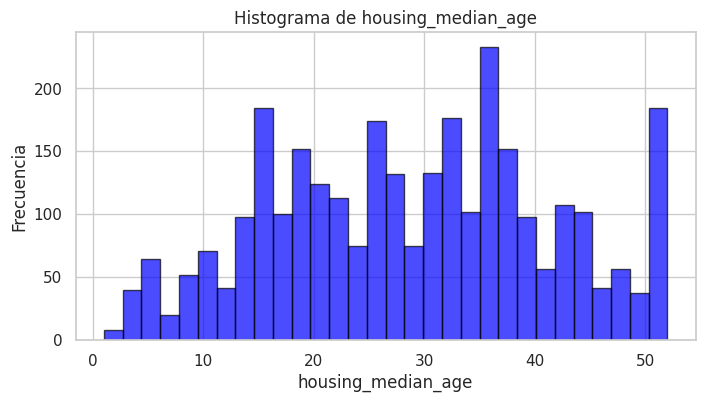
\includegraphics[width=0.8\textwidth]{graficas/housing_median_age.png}
\caption{Histograma de \texttt{housing\_median\_age}.}
\label{fig:hist_age}
\end{figure}

\begin{figure}[ht]
\centering
\includegraphics[width=0.8\textwidth]{graficas/correlación.png}
\caption{Gráficos de dispersión para \texttt{median\_house\_value}, \texttt{total\_rooms} y \texttt{total\_bedrooms}.}
\label{fig:dispersion}
\end{figure}

\begin{figure}[ht]
\centering
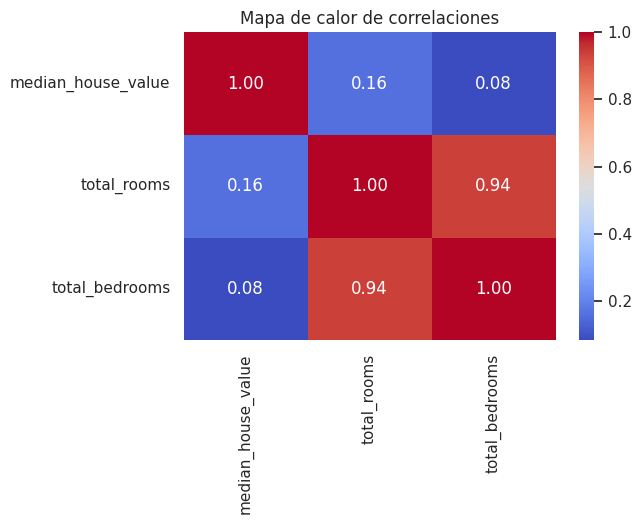
\includegraphics[width=0.8\textwidth]{graficas/mapacalor.png}
\caption{Mapa de calor de la matriz de correlación.}
\label{fig:heatmap}
\end{figure}

\section{Análisis e Interpretación}\label{s:5}
\subsection{Análisis Univariado}
La Figura~\ref{fig:hist_age} ilustra la distribución de la variable \texttt{housing\_median\_age}. Se observa que la mayoría de las viviendas tienen edades concentradas en un rango específico. Las medidas de tendencia central y dispersión permiten identificar el comportamiento típico y la variabilidad de la distribución.

\subsection{Análisis Bivariado}
Los gráficos de dispersión (Figura~\ref{fig:dispersion}) muestran relaciones claras entre el valor mediano de las viviendas y el número de habitaciones, sugiriendo una correlación positiva. Asimismo, el mapa de calor (Figura~\ref{fig:heatmap}) confirma una alta correlación entre \texttt{total\_rooms} y \texttt{total\_bedrooms}, lo cual respalda la hipótesis de que, a mayor cantidad de habitaciones, se incrementa el número de dormitorios.

\section{Conclusiones}\label{s:6}
El estudio realizado permite concluir que:
\begin{itemize}
    \item El análisis univariado revela la distribución y dispersión de cada variable, facilitando la comprensión de la estructura del dataset.
    \item El análisis bivariado indica relaciones significativas entre el tamaño de las viviendas y su valor, lo que puede servir como base para modelos predictivos.
\end{itemize}



\end{document}
